%!TEX root = ../preamble.tex

\section{Results}
\label{sec:results}

\subsection{Experiments with the convolutional neural network}


\subsubsection{Feature maps}
The feature maps shown on figure \ref{fig:featuremaps} are visualised by scaling the output range of $[0,1]$ of every neuron linearly to the grey scale range of $[0,255]$. The leftmost column of feature maps are from the first convolutional layer, and the rightmost is the input to the fully connected layers. As a convolutional layer takes a depth slice of all the previous feature maps as input, their is no apparent connection between the visualised output of the max pooling layer and the following result of the convolutional layer.

\begin{figure}[H]
	\begin{scriptsize}
		\sffamily
		\def\svgwidth{\textwidth}
		\input{img/featuremaps.pdf_tex}
	\end{scriptsize}
	\caption{A small subset of the feature maps produced from running a training example from the lightened arena through the visual partitioning classification deep convolutional neural network. The feature maps highlight the position of the target.}
	\label{fig:featuremaps}
\end{figure}

%Shallow vs deep
%No light vs light

%%!TEX root = ../preamble.tex

\pgfplotstableread{data/nolight-angular-shallow.dat}{\nolightAngularShallow}
\pgfplotstableread{data/nolight-angular-deep.dat}{\nolightAngularDeep}

\begin{figure}[H]
\begin{tikzpicture}[scale=1]
	\begin{axis}[
			title=Score over iterations,
			xlabel=Iterations,
			ylabel=Score,
			xmin = -640,
			xmax = 16640,
			restrict x to domain=0:16000,
			xticklabel style={rotate=30},
			minor x tick num=1,
			legend pos=north east,
		]
		\addplot+ [cred, mark=none] table [x={iteration}, y={score}] {\nolightAngularShallow};
		\addlegendentry{Shallow architecture}
		\addplot+ [cblue, mark=none] table [x={iteration}, y={score}] {\nolightAngularDeep};
		\addlegendentry{Deep architecture}
	\end{axis}
\end{tikzpicture}
\caption{Training convolutional neural networks using angular regression without visual distortion}
\end{figure} %DONE
%%!TEX root = ../preamble.tex

\pgfplotstableread{data/nolight-deep.dat}{\nolightDeep}
\begin{figure}[H]
\begin{tikzpicture}[scale=1]
	\begin{axis}[
			title=Score over iterations,
			xlabel=Iterations,
			ylabel=Score,
			xmin = -480,
			xmax = 12480,
			restrict x to domain=0:12000,
			xticklabel style={rotate=30},
		]
		\addplot+ [cred, mark=none] table [x={iteration}, y={score}] {\nolightDeep};
	\end{axis}
\end{tikzpicture}
\caption{Training of a deep convolutional network without lights}
\end{figure}
%%!TEX root = ../preamble.tex

\pgfplotstableread{data/nolight-shallow.dat}{\nolightShallow}
\begin{figure}[H]
\begin{tikzpicture}[scale=1]
	\begin{axis}[
			title=Score over iterations,
			xlabel=Iterations,
			ylabel=Score,
			restrict x to domain=0:6000,
			enlarge x limits=0.1,
		]
		\addplot+ [red, mark=none] table [x={iteration}, y={score}] {\nolightShallow};
	\end{axis}
\end{tikzpicture}
\caption{Training of a shallow convolutional network without lights}
\end{figure} %DONE

%%!TEX root = ../preamble.tex

\pgfplotstableread{data/light-angular.dat}{\lightAngular}
\begin{figure}[H]
\begin{tikzpicture}[scale=1]
	\begin{axis}[
			xlabel=Iterations,
			ylabel=Score,
			xmin = -640,
			xmax = 16640,
			restrict x to domain=0:16000,
			xticklabel style={rotate=30},
			minor x tick num=1,
		]
		\addplot+ [red, mark=none] table [x={iteration}, y={score}] {\lightAngular};
	\end{axis}
\end{tikzpicture}
\caption{Training of a deep convolutional network to detect angles and distance with light}
\end{figure}
%%!TEX root = ../preamble.tex

\pgfplotstableread{data/light-deep.dat}{\lightDeep}
\begin{figure}[H]
\begin{tikzpicture}[scale=1]
	\begin{axis}[
			title=Score over iterations training a deep convolutional network with lights,
			xlabel=Iterations,
			ylabel=Score,
			xmin = -480,
			xmax = 12480,
			restrict x to domain=0:12000,
			xticklabel style={rotate=30},
		]
		\addplot+ [red, mark=none] table [x={iteration}, y={score}] {\lightDeep};
	\end{axis}
\end{tikzpicture}
\caption{Score over iterations training a deep convolutional network with lights}
\end{figure} %DONE
%%!TEX root = ../preamble.tex

\pgfplotstableread{data/light-shallow.dat}{\lightShallow}
\begin{figure}[H]
\begin{tikzpicture}[scale=1]
	\begin{axis}[
			title=Score over iterations training a shallow convolutional network with lights,
			xlabel=Iterations,
			ylabel=Score,
			xmin = -500,
			xmax = 12500,
			restrict x to domain=0:12000,
			xticklabel style={rotate=30},
		]
		\addplot+ [cred, mark=none] table [x={iteration}, y={score}] {\lightShallow};
	\end{axis}
\end{tikzpicture}
\caption{Score over iterations training a shallow convolutional network with lights}
\end{figure}

%!TEX root = ../preamble.tex






\definecolor{cpurple}{HTML}{BA6FB6}
\definecolor{corange}{HTML}{FDAE61}
\definecolor{cgreen}{HTML}{ABDDA4}
\definecolor{cblue}{HTML}{2B83BA}

\begin{figure}[H]
\centering
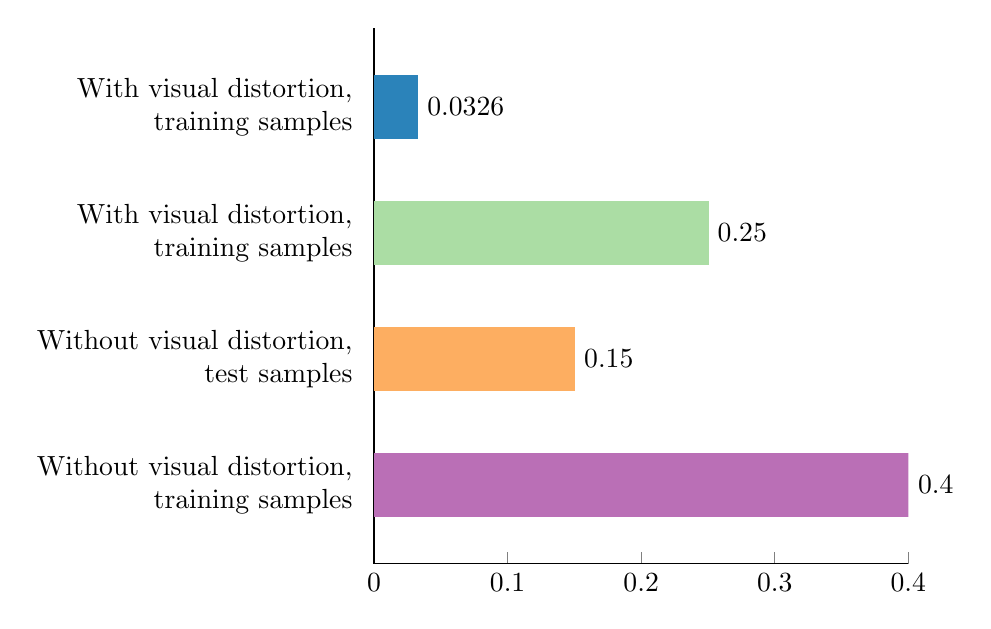
\begin{tikzpicture}
\begin{axis}[
    xbar=0pt,
    /pgf/bar shift=0pt,
    legend style={
    legend columns=4,
        at={(xticklabel cs:0.5)},
        anchor=north,
        draw=none
    },
    ytick={0,...,3},
    ytick style={draw=none},
    axis y line*=none,
    axis x line*=bottom,
    xtick={0,0.1,...,0.5},
    width=.69\textwidth,
    bar width=8mm,
	yticklabels={	{Without visual distortion,\\training samples}, 
						{Without visual distortion,\\test samples}, 
						{With visual distortion,\\training samples}, 
						{With visual distortion,\\training samples}, 
	},
	yticklabel style={align=right},
    xmin=0,
    xmax=0.4,
    area legend,
    y=16mm,
    enlarge y limits={abs=0.625},
    nodes near coords,
    every node near coord/.style={/pgf/number format/fixed, /pgf/number format/precision=5, text=black},
    every axis plot/.append style={fill}
]
\addplot[cpurple] coordinates {(0.400,0)};
\addplot[corange] coordinates {(0.150,1)};
\addplot[cgreen] coordinates {(0.250,2)};
\addplot[cblue] coordinates {(0.0326,3)};
\end{axis}  
\end{tikzpicture}
\caption{X}
\label{fig:stats}
\end{figure}

















































